\documentclass[12pt,a4paper,oneside]{article}
\usepackage[utf8]{inputenc}
\usepackage[english]{babel}
\usepackage{amsmath}
\usepackage{amsfonts}
\usepackage{amssymb}
\usepackage{graphicx}
\usepackage{multirow}
\usepackage{longtable}
\usepackage[left=3cm,right=2cm,top=3cm,bottom=2cm]{geometry}
\begin{document}

\begin{center}
\textbf{\large{Context Description and Next Activities}}
\end{center}
\bigskip

\begin{figure}[b!]
\center
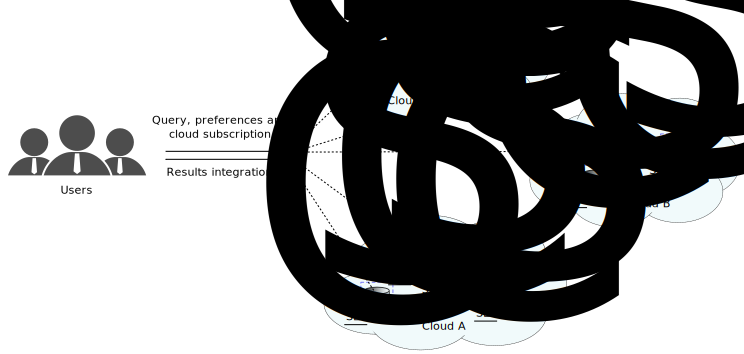
\includegraphics[scale=1]{figures/scenario.pdf}\caption{Data integration context overview}\label{fig:context}
\end{figure}

The figure~\ref{fig:context} illustrates our data integration scenario. Cloud providers (for instance, Cloud Provider A, Cloud Provider B and Cloud Provider C) offer cloud resources to data providers (for instance, Data provider 1, Data provider 2, Data provider 3 and Data provider 4) willing to deploy their services. The cloud provider and the data service establish a contract specifying what guarantees in terms of infrastructure resources (for instance, storage limit, memory limit, processing capacity) the data service can expect from the cloud. This contract is called \textsl{Cloud SLA} ($SLA_{C}$).

Data services can deploy services in the clouds they have subscriptions respecting what is agreed in the $SLA_{C}$. Each service deployed by the data service in the cloud export a different SLA (called \textsl{Service SLA} - $SLA_{S}$) which specifies what service customers can expect in terms of data quality guarantees (for instance, provenance, freshness, data type, degree of rawness) from its service. The data provider defines the $SLA_{S}$ for the services deployed on a cloud according to what it is defined in the $SLA_{C}$. For instance, considering that a \textsl{data provider} have agreed with a \textsl{cloud provider} to have limit of 10 gigabytes of free data transferred per day, the \textsl{data provider} could define on his $SLA_{S}$ that he can perform 300 requests per day, and each request costs 0.1\$. In other words, the $SLA_{S}$ guarantees are derived from the $SLA_{C}$. Moreover, a \textsl{data provider} can deploy the same service in different clouds in which he has established contracts (for instance, the \textsl{Data provider} 1 deployed the service S1 in the clouds A and B) and for each different \textsl{Cloud provider} a different $SLA_{S}$ is defined for the same service.

The end-user willing to integrate data interacts with our \textsl{Data Integration-as-a-Service} (\textsl{DIaaS}). The \textsl{DIaaS} is responsible to select and match the services that can produce the result expected by the user according to his preferences, where he is consuming the data, and the different SLAs associated to the services and to the cloud providers. Once the composition is created and executed, the integration results are delivered to the user and an \textsl{integration SLA} ($SLA_{I}$) is established. This SLA is responsible to include information collected during the integration process which can be reused in a further integration request.

\section{Basic concepts}

A user willing to perform a data integration task defines \textit{(i)} a \textsl{query}; and \textit{(ii)} a set of  \textsl{requirements} over the services or/and over the entire composition (integration). \textsl{Queries} are specified in terms of \textsl{abstract services}' definitions.

% ----------------------------------- DEFINITION 1 ABSTRACT SERVICE --------------------------------- %
\bigskip
\noindent \textbf{Definition 1 (\textsl{Abstract service})}. An \textsl{abstract service} describes the small piece of function performed by a \textsl{service} deployed by a \textsl{data provider}. For instance, retrieve weather information, book a hotel, retrieve infected patients, among others. The \textsl{abstract service} is defined as follows: $A \ (\overline{I}; \ \overline{O})$ where $A$ is the name which identifies the \textsl{abstract service}. $\overline{I}$ and $\overline{O}$ are a set of comma-separated input and output parameters, respectively.

% ----------------------------------- DEFINITION 2 QUERY --------------------------------- %
\bigskip
\noindent \textbf{Definition 2 (\textsl{Query})}.
An user \textsl{query} $Q$ is defined as a sequence of \textsl{abstract services} followed by a set of \textsl{user requirements} in accordance with the grammar:
%
\begin{center}
\begin{math}
Q (\overline{I}_{h}; \overline{O}_{h}) := A_{1}(\overline{I}_{1l};
\overline{O}_{1l}), A_{2}(\overline{I}_{2l}; \overline{O}_{2l}), ..,  A_{n}(\overline{I}_{nl}; \overline{O}_{nl}),R_{1},R_{2}, .., R_{m}
\end{math}
\end{center}
%

The \textsl{query} is defined in terms of \textsl{abstract services} ($A_{1}, A_{2}, .., A_{n}$) including a set of \textsl{user requirements} ($R_{1},R_{2}, .., R_{m}$). 
The left-hand of the definition is called the \textit{head}; it defines \textsl{query} name $Q$, a set of input $\overline{I}$ and output $\overline{O}$ variables, respectively. Variables in the \textit{head} are identified by $\overline{I}_{h}$ and $\overline{O}_{h}$, and they are called \textit{head} variables. The right-hand is the \textit{body} definition; it includes a set of \textsl{abstract services} followed by a set of \textsl{user requirements}. \textsl{Abstract services} in the \textit{body} also defines input and output variables. Variables appearing in the \textit{body} are identified by $\overline{I}_{l}$ and $\overline{O}_{l}$. \textit{Head} variables can appear in the \textit{body}, and variables appearing only in the \textit{body} are called \textit{local} variables.
%\textit{Head} variables can be accessed and shared among different services. On the other hand, \textit{local} variables can be used only by the service which define them.
%The left-hand of the definition is called the \textit{head}; and the right-hand is the \textit{body}. 
%A \textsl{query} $Q$ includes a set of input $\overline{I}$ and output $\overline{O}$ variables, respectively.
%Variables in the \textit{head} are identified by $\overline{I}_{h}$ and $\overline{O}_{h}$, and called \textit{head} variables. 
%They appear in the \textit{head} and in the \textit{body} definition. 
%Variables appearing only in the \textit{body} are identified by $\overline{I}_{l}$ and $\overline{O}_{l}$, and are called \textit{local} variables. \textit{Head} variables can be accessed and shared among different services. On the other hand, \textit{local} variables can be used only by the service which define them.
%

\bigskip
In order to be able to compare queries, we assume that there is an ontology (like the one used in~\cite{Barhamgi2010}) to describe the \textsl{abstract services} semantics. The comparison between \textsl{queries} is allowed by the query containment concept.

% ----------------------------------- DEFINITION 3 QUERY CONTAINMENT --------------------------------- %
\bigskip
\noindent \textbf{Definition 3 (\textsl{Query containment})}.
A \textsl{query} $Q_{1}$ is contained in a \textsl{query} $Q_{2}$, denoted by $Q_{1} \subset Q_{2}$, if and only if the result to $Q_{1}$ is a subset of the result to $Q_{2}$.
%

\bigskip
Intuitively, the query equivalence is defined as follows:

% ----------------------------------- DEFINITION 4 QUERY CONTAINMENT --------------------------------- %
\bigskip
\noindent \textbf{Definition 4 (\textsl{Query equivalence})}.
A \textsl{query} $Q_{1}$ is equivalent to a \textsl{query} $Q_{2}$, denoted by $Q_{1} \equiv Q_{2}$, if and only if $Q_{1} \subset Q_{2}$ and $Q_{2} \subset Q_{1}$.
%

% ----------------------------------- DEFINITION 3 USER REQUIREMENTS --------------------------------- %
\bigskip
\noindent \textbf{Definition 5 (\textsl{User requirement})}.
An \textsl{user requirement} $r$ is in the form $x \otimes c$, where $x$ is an identifier; $c$ is a constant; and $\otimes \in\lbrace \geq, \leq, =, \neq, <, >\rbrace$. 
%
The \textsl{user requirement} $r$ could concern \textit{(i)} the entire \textsl{query}, in this case noted as $r_{Q}$; or \textit{(ii)} a single \textsl{service}, noted as $r_{S}$. For instance, the \textsl{total response time} is obtained by adding the \textsl{response time} of each \textsl{service} involved in the composition.

% ----------------------------------- DEFINITION 4 USER REQUIREMENTS DOMAIN --------------------------------- %
\bigskip
\noindent \textbf{Definition 6 (\textsl{Requirement domain})}. A \textsl{requirement domain} is a set of possible values which can be assumed by an \textsl{user requirement} $r$, represented by $Dom(r)$. For instance, a \textsl{requirement domain} ``\textit{response time}'' includes the possible values associated to the \textit{response time} \textsl{user requirement}. Each \textsl{user requirement} $r_{i}$ has its own \textsl{requirement domain} $D_{i}$. 

% ----------------------------------- DEFINITION 5 EVALUATION --------------------------------- %
\bigskip
\noindent \textbf{Definition 7 (\textsl{User requirement evaluation})}. The evaluation of an \textsl{user requirement} $r$, indicated by $eval(r)$, returns a set of values $\lbrace v_{1},..,v_{i} \rbrace$ that can be assigned to $r$ such that $\lbrace v_{1},..,v_{i} \rbrace \subset Dom(r)$.

% ----------------------------------- DEFINITION 6 COMPARABLE REQUIREMENTS --------------------------------- %
\bigskip
\noindent \textbf{Definition 8 (\textsl{Comparable requirements})}. Given two \textsl{user requirements} $r_{1}$ and $r_{2}$, both can be comparable, denoted by $r_{1} \perp r_{2}$, if and only if:  $Dom(r_{1}) = Dom(r_{2})$.

% ----------------------------------- DEFINITION 7 REQUIREMENTS EQUIVALENCE --------------------------------- %
\bigskip
\noindent \textbf{Definition 9 (\textsl{User requirements equivalence})}.
A set of \textsl{user requirements} $R_{1}$ is equivalent to a set of \textsl{user requirements} $R_{2}$, represented by $R_{1} \equiv R_{2}$, if and only if: $\forall r_{i} \in R_{1}, \ \exists r_{j} \in R_{2} \ \vert \ eval (r_{i}) = eval(r_{j}) \ and \ \vert R_{1} \vert = \vert R_{2} \vert$.

% ----------------------------------- DEFINITION 8 REQUIREMENTS MORE RESTRICT --------------------------------- %
\bigskip
\noindent \textbf{Definition 10 (\textsl{User requirements more restrict})}.
Given a set of \textsl{user requirements} $R_{1}$ and $R_{2}$, $R_{1}$ is more restrict than $R_{2}$, represented by $R_{1} \ \rhd \ R_{2}$, if and only if:
\begin{flushleft}
Case 1: $\forall r_{i} \in R_{1}, \ \exists r_{j} \in R_{2}, \ \nexists r_{k} \in R_{2} \ \vert \ eval (r_{i}) \subset eval(r_{j}) \ and \ eval (r_{k}) \subset eval(r_{i}) \ and \ \vert R_{1} \vert = \vert R_{2} \vert$.
\end{flushleft}
\begin{flushleft}
Case 2: $\forall r_{i} \in R_{1}, \ \exists r_{j} \in R_{1}, \ \exists r_{k} \in R_{2}, \ \nexists r_{l} \in R_{2} \ \vert \ \neg (r_{j} \ \bot \ r_{k}) \ and \ eval (r_{l}) \subset eval(r_{i})$.
\end{flushleft}
%\begin{flushleft}
%Case 3: $\forall r_{i} \in R_{1}, \ \exists r_{j} \in R_{2} \ \vert \ eval (r_{i}) \supset eval(r_{j}) \ and \ \vert R_{1} \vert > \vert R_{2} \vert$. 
%\end{flushleft}

% ----------------------------------- DEFINITION 9 REQUIREMENTS LESS RESTRICT --------------------------------- %
%\bigskip
%\noindent \textbf{Definition 9 (\textsl{User requirements less restrict})}.
%Given a set of \textsl{user requirements} $R_{1}$ and $R_{2}$, $R_{1}$ is less restrict than $R_{2}$, represented by $R_{1} \ \lhd \ R_{2}$, if and only if:
%\begin{flushleft}
%Case 1: $\forall r_{i} \in R_{1}, \ \exists r_{j} \in R_{2} \ \vert \ eval (r_{i}) \supset eval(r_{j}) \ and \ \vert R_{1} \vert = \vert R_{2} \vert$.
%\end{flushleft}
%\begin{flushleft}
%Case 2: $\forall r_{j} \in R_{2}, \ \exists r_{i} \in R_{1} \ \vert \ eval (r_{j}) \subset eval(r_{i}) \ and \ \vert R_{1} \vert < \vert R_{2} \vert$.
%\end{flushleft}

% ----------------------------------- DEFINITION 10 PART MORE / LESS RESTRICT --------------------------------- %
\bigskip
\noindent \textbf{Definition 11 (\textsl{Part of the user requirements more restrict and part less restrict})}.
Given a set of \textsl{user requirements} $R_{1}$ and $R_{2}$, part of the \textsl{user requirements} $R_{1}$ can be more restrict and part less restrict than the \textsl{user requirements} $R_{2}$, represented by $R_{1} \ \diamond \ R_{2}$, if and only if:
\begin{flushleft}
$\forall r_{i} \in R_{1}, \ \exists r_{j} \in R_{2} \ \vert \ (eval (r_{i}) \subset eval(r_{j}) \ or \ eval (r_{i}) \supset eval(r_{j})) \ and \ \vert R_{1} \vert = \vert R_{2} \vert$.
\end{flushleft}

% ----------------------------------- DEFINITION 11 REQUIREMENTS COMPLETELY DIFFERENT --------------------------------- %
\bigskip
\noindent \textbf{Definition 12 (\textsl{User requirements different})}.
Given a set of \textsl{user requirements} $R_{1}$ and $R_{2}$, $R_{1}$ is different of $R_{2}$, represented by $R_{1} \ \neq \ R_{2}$, if and only if:
\begin{flushleft}
$\forall r_{i} \in R_{1}, \ \nexists r_{j} \in R_{2} \ \vert \ eval (r_{i}) \subset eval(r_{j}) \ or \ eval (r_{i}) \supset eval(r_{j})$.
\end{flushleft}
%
%% ----------------------------------- DEFINITION 7 QUERY EQUIVALENCE  --------------------------------- %
%\bigskip
%\noindent \textbf{Definition 11 (\textsl{Query equivalence})}.
%Definition 2 (query equivalence): a query Q1 is equivalent to a query Q2 if: 
%Q1 and Q2 have the same number of abstract services
%For each abstract services in Q1 there is an equivalent in Q2
%
%% ----------------------------------- DEFINITION 8 QUERY SUBSET  --------------------------------- %
%\bigskip
%\noindent \textbf{Definition 12 (\textsl{Query subset})}.
%Definition 10 (query subset): a query Q1 is a subset of the query Q2 if: 
%Q1 has less abstract services than Q2
%For each abstract service in Q1 there is an equivalent in Q2.
%In other words, the query Q1 is contained in the query Q2.
%
%% ----------------------------------- DEFINITION 9 QUERY ??  --------------------------------- %
%\bigskip
%\noindent \textbf{Definition 13 (\textsl{different queries but with some abstract services in common})}.
%Definition 11 (different queries but with some abstract services in common): this case occurs when given a query Q1 and a query Q2: 
%Q1 and Q2 have a different number of abstract services
%There is at least one abstract service in Q1 that has an equivalent in Q2;
%There is at least one abstract service in Q1 that has no equivalent in Q2; and
%There is at least one abstract service in Q2 that has no equivalent in Q1;


\section{Taxonomy of query variations for promoting the reusability of rewriting results}

This section describes the different types of queries which \textit{(i)} can be processed by our integration approach; or \textit{(ii)} can be compared to previous integration requests in order to take advantage from previous integration plans.

Examples illustrate each kind of query and the reusability solution. 
The table~\ref{table:abstractservices} introduces the \textsl{abstract services} used in the examples according to our medical scenario. Four \textsl{abstract services} are used for defining the queries and \textsl{concrete services}.



\begin{table}[!ht]
\center
\begin{tabular}{|>{\raggedright\arraybackslash}p{4cm}|>{\raggedright\arraybackslash}p{8cm}|}
\hline 
\textsl{\textbf{Abstract service}} & \textit{\textbf{Description}} \\ 
\hline 
$A_{1} (x?; y!)$ & Given a disease $x$, $A_{1}$ returns the list of patients $p$ that were infected by it. \\ 
\hline 
$A_{2} (z?; w!)$ & Given a patient id $z$, $A_{2}$ returns his/her personal information $w$. \\ 
\hline 
$A_{3} (d?; y!)$ & Given a doctor id $d$, $A_{3}$ returns the list of patients $y$ that were treated by $d$. \\ 
\hline 
$A_{4} (h?; y!)$ & Given a hospital $h$, $A_{4}$ returns the list of patients $y$ that were treated in it. \\ 
\hline  
\end{tabular}\label{table:abstractservices}
\end{table}

\begin{example}\label{example:query}
To better understand the taxonomy of queries and the reusability solution, let us consider a previous integration request processed by doctor Marcel. \textit{He has searched for patients infected by pneumonia that were treated by doctor Paul using services with availability higher than 97\%, response time less than 3 seconds, price per call less than 2 cents, certified data providers, fresh data or not, the overall response time less than 10 seconds and the total cost less than 5 dollars}. This query can be expressed according to the grammar (defined in the section~\ref{idk}) as follows:
\begin{flushleft}
$\hspace{1cm} Q_{p} \ (disaese?, \ doctor?; \ p\_information!) \ := \ A_{1} (disease?; \ p!), \ A_{3} (doctor?; \ p!),$ \\ 
$ \hspace{2cm} \ A_{2} (p?; \ p\_information!), \ availability > 97\%, \ response \ time < 3s,$ \\ 
$ \hspace{2cm} \ price \ per \ call < 0.2\$, \ provenance = certified, \ freshness = no,$ \\ 
$ \hspace{2cm} \ total \ response \ time < 10s, \ total \ cost < 5\$$
\end{flushleft}
\end{example}
 
The following subsections describe the queries variation and their reusability solution. For all query variation described bellow, we assume a previous integration request defining the \textsl{query} $Q_{p}$ including its \textsl{user requirements} $R_{p}$ as presented in the Example~\ref{example:query}.

\subsection{Case 1: Equivalent \textsl{query} and equivalent \textsl{user requirements}}
Given a user request defining a \textsl{query} $Q_{n}$ and a set of \textsl{requirements} $R_{n}$, the case in which the \textsl{queries} and the \textsl{requirements} are equivalent occurs if and only if: $Q_{n} \equiv Q_{p}$ and $R_{n} \equiv R_{p}$ (Figure \ref{fig:case1}).

\begin{figure}[h!]
\center
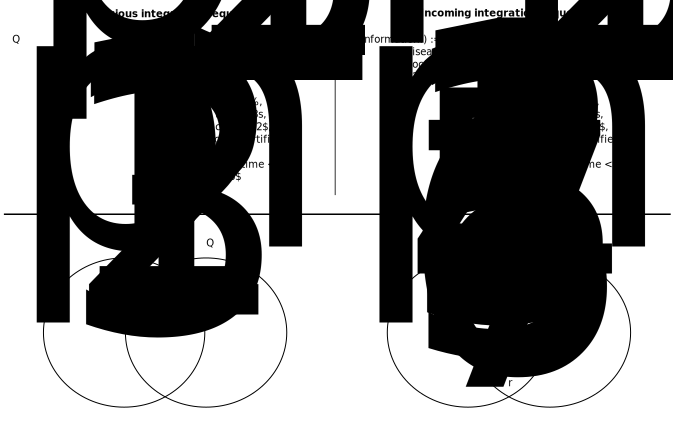
\includegraphics[scale=0.85]{figures/query-case-1.pdf}\caption{Query case 1} \label{fig:case1}
\end{figure}

\bigskip
\noindent \textbf{Solution:} This is the best case processed by our data integration approach. There are three possible workflows: First, if all involved \textsl{concrete services} could be enforced according to their available resources, the previous composition could be re-executed. Then, a new \textsl{integration SLA} would be produced and stored to the new request. Second, if part of the involved \textsl{concrete services} could not be enforced according to their available resources, these services would be re-allocated by our rewriting algorithm. Once a valid composition is produced, it can be re-executed. Then, a new \textsl{integration SLA} would be produced and stored to the new request. Third, if all involved \textsl{concrete services} could not be enforced according to their available resources, the new \textsl{query} will be dispatched to be rewriting by our rewriting algorithm.

\subsection{Equivalent \textsl{query} and more restrict \textsl{user requirements}}
Given a user request defining a \textsl{query} $Q_{n}$ and a set of \textsl{requirements} $R_{n}$, the case in which the \textsl{queries} are equivalent and the \textsl{requirements} for the new request are more restrict occurs if and only if: $Q_{n} \equiv Q_{p}$ and $R_{n} \triangleright R_{p}$ (See figures \ref{fig:case2a} and \ref{fig:case2b}).

\begin{figure}[h!]
\center
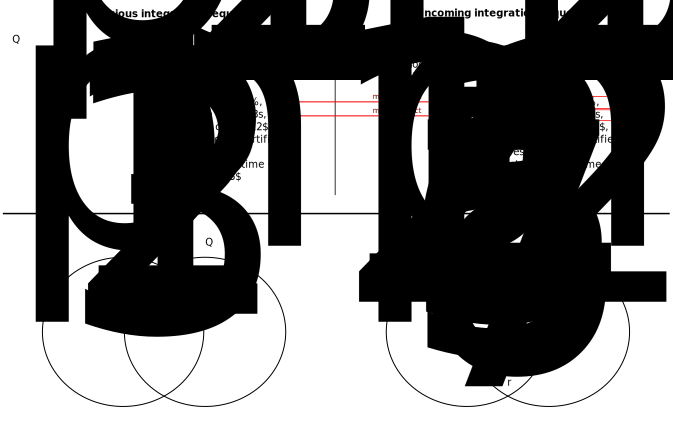
\includegraphics[scale=0.85]{figures/query-case-2a.pdf}\caption{Query case 2a}\label{fig:case2a}
\end{figure}

\begin{figure}[h!]
\center
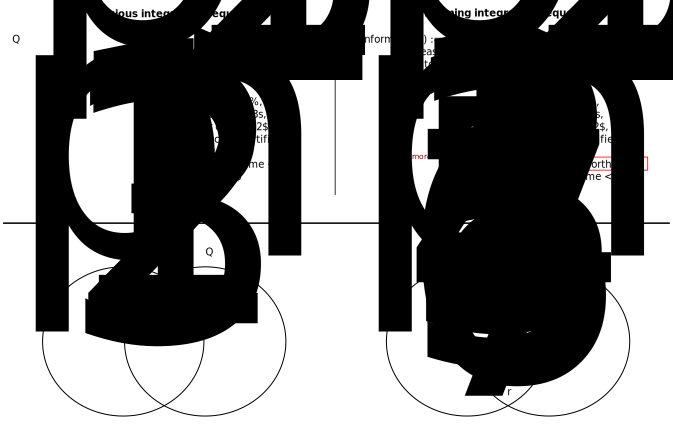
\includegraphics[scale=0.85]{figures/query-case-2b.pdf}\caption{Query case 2b}\label{fig:case2b}
\end{figure}

\bigskip
\noindent \textbf{Solution:} There are three possible workflows: First, if all involved \textsl{concrete services} could be enforced to the new request according to the new requirements and their available resources, the previous composition could be re-executed. Then, a new \textsl{integration SLA} is produced and stored to the new request. Second, if part of the involved \textsl{concrete services} could not be enforced to the new request according to the new requirements and their available resources, these services are re-allocated by our rewriting algorithm. Once a new valid composition is produced, it  could be executed. Then, a new \textsl{integration SLA} is produced and stored to the new request. Third, if all involved \textsl{concrete services} could not be enforced to the new request according to the new requirements and their available resources, the new \textsl{query} is dispatched to our rewriting algorithm. Once a new valid composition is produced, it  could be executed. Then, a new \textsl{integration SLA} is produced and stored to the new request.

\subsection{Equivalent \textsl{query} and less restrict \textsl{user requirements}}
Given a user request defining a \textsl{query} $Q_{n}$ and a set of \textsl{requirements} $R_{n}$, the case in which the \textsl{queries} are equivalent and the \textsl{requirements} for the new request are less restrict occurs if and only if: $Q_{n} \equiv Q_{p}$ and $R_{p} \triangleright R_{n}$ (See figures \ref{fig:case3a} and \ref{fig:case3b}).

\begin{figure}[h!]
\center
\includegraphics[scale=0.85]{figures/query-case-3a.pdf}\caption{Query case 3a} \label{fig:case3a}
\end{figure}

\begin{figure}[h!]
\center
\includegraphics[scale=0.85]{figures/query-case-3b.pdf}\caption{Query case 3b} \label{fig:case3b}
\end{figure}

\bigskip
\noindent \textbf{Solution:}  There are three possible workflows: First, if all involved \textsl{concrete services} could be enforced to the new request according to their available resources, the previous composition could be re-executed. Then, a new \textsl{integration SLA} is produced and stored to the new request. Second, if part of the involved \textsl{concrete services} could not be enforced to the new request according to their available resources, these services are re-allocated by our rewriting algorithm. Once a new valid composition is produced, it could be executed. Then, a new \textsl{integration SLA} is produced and stored to the new request. Third, if all involved \textsl{concrete services} could not be enforced to the new request according to their available resources, the new \textsl{query} is dispatched to our rewriting algorithm. Once a new valid composition is produced, it  could be executed. Then, a new \textsl{integration SLA} is produced and stored to the new request.

\subsection{Equivalent \textsl{queries} and part of the \textsl{user requirements} less restrict and part more restrict}
Given a user request defining a \textsl{query} $Q_{n}$ and a set of \textsl{requirements} $R_{n}$, the case in which the the incoming \textsl{query} is equivalent to the previous \textsl{query} and part of the \textsl{requirements} are more restrict and part less restrict occurs if and only if: $Q_{n} \equiv Q_{p}$ and $R_{n} \diamond R_{p}$ (See figures \ref{fig:case4a}, \ref{fig:case4b} and \ref{fig:case4c}).

\begin{figure}[h!]
\center
\includegraphics[scale=0.85]{figures/query-case-4a.pdf}\caption{Query case 4a} \label{fig:case4a}
\end{figure}

\begin{figure}[h!]
\center
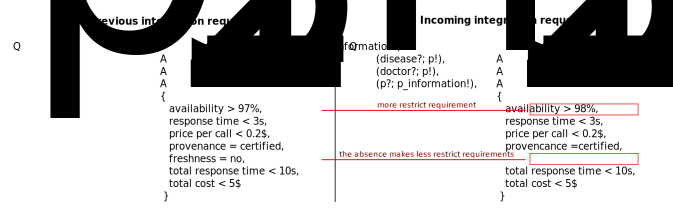
\includegraphics[scale=0.85]{figures/query-case-4b.pdf}\caption{Query case 4b} \label{fig:case4b}
\end{figure}

\begin{figure}[h!]
\center
\includegraphics[scale=0.85]{figures/query-case-4c.pdf}\caption{Query case 4c} \label{fig:case4c}
\end{figure}

\bigskip
\noindent \textbf{Solution:} There are three possible workflows: First, if all involved \textsl{concrete services} could be enforced to the new request according to the new requirements and their available resources, the previous composition could be re-executed. Then, a new \textsl{integration SLA} is produced and stored to the new request. Second, if part of the involved \textsl{concrete services} could not be enforced to the new request according to the new requirements and their available resources, these services are re-allocated by our rewriting algorithm. Once a new valid composition is produced, it  could be executed. Then, a new \textsl{integration SLA} is produced and stored to the new request. Third, if all involved \textsl{concrete services} could not be enforced to the new request according to the new requirements and their available resources, the new \textsl{query} is dispatched to our rewriting algorithm. Once a new valid composition is produced, it  could be executed. Then, a new \textsl{integration SLA} is produced and stored to the new request.

\subsection{Equivalent \textsl{query} and different \textsl{user requirements}}
Given a user request defining a \textsl{query} $Q_{n}$ and a set of \textsl{requirements} $R_{n}$, the case in which the the incoming \textsl{query} is equivalent to the previous \textsl{query} and part of the \textsl{requirements} are more restrict and part less restrict occurs if and only if: $Q_{n} \equiv Q_{p}$ and $R_{n} \neq R_{p}$ (See figure \ref{fig:case5}).

\begin{figure}[h!]
\center
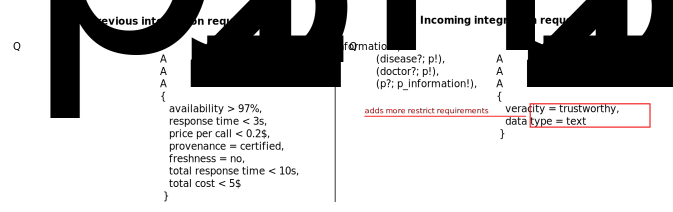
\includegraphics[scale=0.85]{figures/query-case-5.pdf}\caption{Query case 5} \label{fig:case5}
\end{figure}

\bigskip
\noindent \textbf{Solution:} There are three possible workflows: First, if all involved \textsl{concrete services} could be enforced to the new request according to the new requirements and their available resources, the previous composition could be re-executed. Then, a new \textsl{integration SLA} is produced and stored to the new request. Second, if part of the involved \textsl{concrete services} could not be enforced to the new request according to the new requirements and their available resources, these services are re-allocated by our rewriting algorithm. Once a new valid composition is produced, it  could be executed. Then, a new \textsl{integration SLA} is produced and stored to the new request. Third, if all involved \textsl{concrete services} could not be enforced to the new request according to the new requirements and their available resources, the new \textsl{query} is dispatched to our rewriting algorithm. Once a new valid composition is produced, it  could be executed. Then, a new \textsl{integration SLA} is produced and stored to the new request.

\subsection{\textsl{Query} subset and equivalent \textsl{user requirements}}
Given a user request defining a \textsl{query} $Q_{n}$ and a set of \textsl{requirements} $R_{n}$, the case in which the the incoming \textsl{query} is a subset of the previous \textsl{query} and the \textsl{requirements} are equivalent occurs if and only if: $Q_{n} \subset Q_{p}$ and $R_{n} \equiv R_{p}$ (See figure \ref{fig:case6}). 

\begin{figure}[h!]
\center
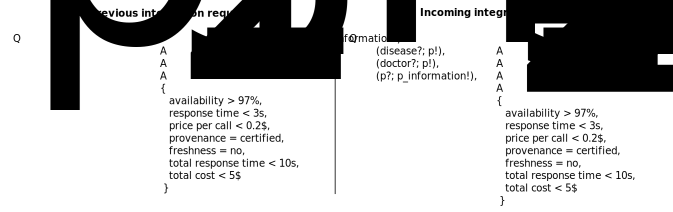
\includegraphics[scale=0.85]{figures/query-case-6.pdf}\caption{Query case 6} \label{fig:case6}
\end{figure}

\bigskip
\noindent \textbf{Solution:} There are three possible workflows: First, if all involved \textsl{concrete services} could be enforced to the new request according to their available resources, the previous composition could be extended to include the service which are missing to achieve the user results. The rewriting algorithm is responsible to select and include this new service. Once a valid composition is produced, it could be executed. Then, a new \textsl{integration SLA} is produced and stored to the new request. Second, if part of the involved \textsl{concrete services} could not be enforced to the new request according to their available resources, these services are re-allocated and the services missing to achieve the user needs are included by our rewriting algorithm. Once a new valid composition is produced, it  could be executed. Then, a new \textsl{integration SLA} is produced and stored to the new request. Third, if all involved \textsl{concrete services} could not be enforced to the new request according to their available resources, the new \textsl{query} is dispatched to our rewriting algorithm. Once a new valid composition is produced, it could be executed. Then, a new \textsl{integration SLA} is produced and stored to the new request.

\subsection{\textsl{Query} subset and more restrict \textsl{user requirements}}
Given a user request defining a \textsl{query} $Q_{n}$ and a set of \textsl{requirements} $R_{n}$, the case in which the the incoming \textsl{query} is a subset of the previous \textsl{query} and the \textsl{requirements} for the new request are more restrict occurs if and only if: $Q_{n} \subset Q_{p}$ and $R_{n} \triangleright R_{p}$ (See figures \ref{fig:case7a} and \ref{fig:case7b}).

\begin{figure}[h!]
\center
\includegraphics[scale=0.85]{figures/query-case-7a.pdf}\caption{Query case 7a} \label{fig:case7a}
\end{figure}

\begin{figure}[h!]
\center
\includegraphics[scale=0.85]{figures/query-case-7b.pdf}\caption{Query case 7b} \label{fig:case7b}
\end{figure}

\bigskip
\noindent \textbf{Solution:} There are three possible workflows: First, if all involved \textsl{concrete services} could be enforced to the new request according to the new \textsl{requirements} and their available resources, the previous composition could be extended to include the services which are missing to achieve the user results. The rewriting algorithm is responsible to select and include new services. Once a valid composition is produced, it could be executed. Then, a new \textsl{integration SLA} is produced and stored to the new request. Second, if part of the involved \textsl{concrete services} could not be enforced to the new request according to the new \textsl{requirements} and their available resources, these services are re-allocated and the services missing to achieve the user needs are included by our rewriting algorithm. Once a new valid composition is produced, it could be executed. Then, a new \textsl{integration SLA} is produced and stored to the new request. Third, if all involved \textsl{concrete services} could not be enforced to the new request according to the new \textsl{requirements} and their available resources, the new \textsl{query} is dispatched to our rewriting algorithm. Once a new valid composition is produced, it could be executed. Then, a new \textsl{integration SLA} is produced and stored to the new request.

\subsection{\textsl{Query} subset and less restrict \textsl{user requirements}}
Given a user request defining a \textsl{query} $Q_{n}$ and a set of \textsl{requirements} $R_{n}$, the case in which the the incoming \textsl{query} is a subset of the previous \textsl{query} and the \textsl{requirements} for the new request are less restrict occurs if and only if: $Q_{n} \subset Q_{p}$ and $R_{p} \triangleright R_{n}$ (See figures \ref{fig:case8a} and \ref{fig:case8b}).

\begin{figure}[h!]
\center
\includegraphics[scale=0.85]{figures/query-case-8a.pdf}\caption{Query case 8a} \label{fig:case8a}
\end{figure}

\begin{figure}[h!]
\center
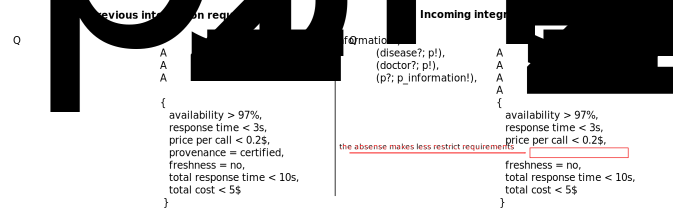
\includegraphics[scale=0.85]{figures/query-case-8b.pdf}\caption{Query case 8b} \label{fig:case8b}
\end{figure}

\bigskip
\noindent \textbf{Solution:} There are three possible workflows: First, if all involved \textsl{concrete services} could be enforced to the new request according to their available resources, the previous composition could be extended to include the services which are missing to achieve the user results. The rewriting algorithm is responsible to select and include new services. Once a valid composition is produced, it could be executed. Then, a new \textsl{integration SLA} is produced and stored to the new request. Second, if part of the involved \textsl{concrete services} could not be enforced to the new request according to their available resources, these services are re-allocated and the services missing to achieve the user needs are included by our rewriting algorithm. Once a new valid composition is produced, it could be executed. Then, a new \textsl{integration SLA} is produced and stored to the new request. Third, if all involved \textsl{concrete services} could not be enforced to the new request according to their available resources, the new \textsl{query} is dispatched to our rewriting algorithm. Once a new valid composition is produced, it could be executed. Then, a new \textsl{integration SLA} is produced and stored to the new request.

\subsection{\textsl{Query} subset and part of the \textsl{user requirements} less restrict and part more restrict}
Given a user request defining a \textsl{query} $Q_{n}$ and a set of \textsl{requirements} $R_{n}$, the case in which the the incoming \textsl{query} is a subset of the previous \textsl{query} and the \textsl{requirements} for the new request are less restrict occurs if and only if: $Q_{n} \subset Q_{p}$ and $R_{p} \diamond R_{n}$ (See figures \ref{fig:case9a} and \ref{fig:case9b}, \ref{fig:case9c}).

\begin{figure}[h!]
\center
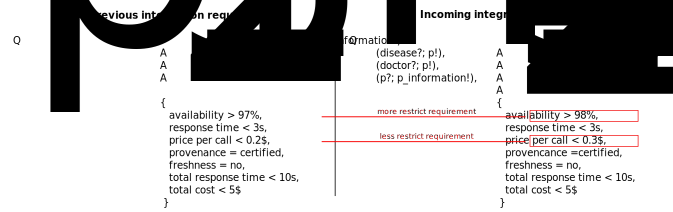
\includegraphics[scale=0.85]{figures/query-case-9a.pdf}\caption{Query case 9a} \label{fig:case9a}
\end{figure}

\begin{figure}[h!]
\center
\includegraphics[scale=0.85]{figures/query-case-9b.pdf}\caption{Query case 9b} \label{fig:case9b}
\end{figure}

\begin{figure}[h!]
\center
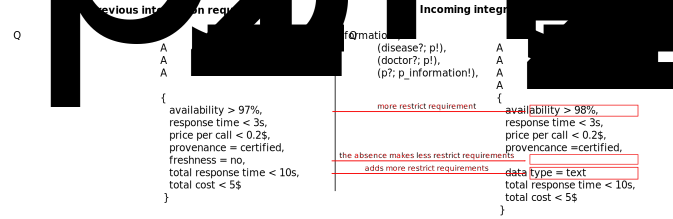
\includegraphics[scale=0.85]{figures/query-case-9c.pdf}\caption{Query case 9c} \label{fig:case9c}
\end{figure}

\bigskip
\noindent \textbf{Solution:} There are three possible workflows: First, if all involved \textsl{concrete services} could be enforced to the new request according to the new \textsl{requirements} and their available resources, the previous composition could be extended to include the services which are missing to achieve the user results. The rewriting algorithm is responsible to select and include new services. Once a valid composition is produced, it could be executed. Then, a new \textsl{integration SLA} is produced and stored to the new request. Second, if part of the involved \textsl{concrete services} could not be enforced to the new request according to the new \textsl{requirements} and their available resources, these services are re-allocated and the services missing to achieve the user needs are included by our rewriting algorithm. Once a new valid composition is produced, it could be executed. Then, a new \textsl{integration SLA} is produced and stored to the new request. Third, if all involved \textsl{concrete services} could not be enforced to the new request according to the new \textsl{requirements} and their available resources, the new \textsl{query} is dispatched to our rewriting algorithm. Once a new valid composition is produced, it could be executed. Then, a new \textsl{integration SLA} is produced and stored to the new request.

\subsection{\textsl{Query} subset and different \textsl{user requirements}}
Given a user request defining a \textsl{query} $Q_{n}$ and a set of \textsl{requirements} $R_{n}$, the case in which the the incoming \textsl{query} is a subset of the previous \textsl{query} and the \textsl{requirements} for the new request are less restrict occurs if and only if: $Q_{n} \subset Q_{p}$ and $R_{p} \neq R_{n}$ (See figure \ref{fig:case10}).

\begin{figure}[h!]
\center
\includegraphics[scale=0.85]{figures/query-case-10.pdf}\caption{Query case 10} \label{fig:case10}
\end{figure}

\bigskip
\noindent \textbf{Solution:} There are three possible workflows: First, if all involved \textsl{concrete services} could be enforced to the new request according to the new \textsl{requirements} and their available resources, the previous composition could be extended to include the services which are missing to achieve the user results. The rewriting algorithm is responsible to select and include new services. Once a valid composition is produced, it could be executed. Then, a new \textsl{integration SLA} is produced and stored to the new request. Second, if part of the involved \textsl{concrete services} could not be enforced to the new request according to the new \textsl{requirements} and their available resources, these services are re-allocated and the services missing to achieve the user needs are included by our rewriting algorithm. Once a new valid composition is produced, it could be executed. Then, a new \textsl{integration SLA} is produced and stored to the new request. Third, if all involved \textsl{concrete services} could not be enforced to the new request according to the new \textsl{requirements} and their available resources, the new \textsl{query} is dispatched to our rewriting algorithm. Once a new valid composition is produced, it could be executed. Then, a new \textsl{integration SLA} is produced and stored to the new request.

\subsection{\textsl{Query} superset and equivalent \textsl{user requirements}}
Given a user request defining a \textsl{query} $Q_{n}$ and a set of \textsl{requirements} $R_{n}$, the case in which the the incoming \textsl{query} is a superset of the previous \textsl{query} and the \textsl{requirements} are equivalent occurs if and only if: $Q_{p} \subset Q_{n}$ and $R_{n} \equiv R_{p}$ (See figure \ref{fig:case11}).

\begin{figure}[h!]
\center
\includegraphics[scale=0.85]{figures/query-case-11.pdf}\caption{Query case 11} \label{fig:case11}
\end{figure}

\bigskip
\noindent \textbf{Solution:} There are three possible solutions for this case. First, if the services used in $Q_{p}$ which are interesting for the \textsl{query} $Q_{n}$ could be correctly mapped and enforced according to the resources available, they could be composed and executed. Second, if part of the services  used in $Q_{p}$ which are interesting for the \textsl{query} $Q_{n}$ could be correctly mapped and enforced according to the resources available, it will be reused. However, the other services necessary to achieve the results will be selected and composed using our rewriting algorithm. Then, when the final composition is produced in accordance with the new \textsl{requirements}, it can be executed. And, third, if none of the services used in $Q_{p}$ which are interesting for the \textsl{query} $Q_{n}$ could be correctly mapped and enforced according to the resources available, the new \textsl{query} will be dispatched to our rewriting algorithm to produce a valid rewriting for this request.

\subsection{\textsl{Query} superset and more restrict \textsl{user requirements}}
Given a user request defining a \textsl{query} $Q_{n}$ and a set of \textsl{requirements} $R_{n}$, the case in which the the incoming \textsl{query} is a superset of the previous \textsl{query} and the \textsl{requirements} for the new request are more restrict occurs if and only if: $Q_{p} \subset Q_{n}$ and $R_{n} \triangleright R_{p}$ (See figures \ref{fig:case12a} and \ref{fig:case12b}.

\begin{figure}[h!]
\center
\includegraphics[scale=0.85]{figures/query-case-12a.pdf}\caption{Query case 12a} \label{fig:case12a}
\end{figure}

\begin{figure}[h!]
\center
\includegraphics[scale=0.85]{figures/query-case-12b.pdf}\caption{Query case 12b} \label{fig:case12b}
\end{figure}

\bigskip
\noindent \textbf{Solution:} There are three possible solutions for this case. First, if the services used in $Q_{p}$ which are interesting for the \textsl{query} $Q_{n}$ could be correctly mapped and enforced according to the new \textsl{requirements} and the resources available, they could be composed and executed. Second, if part of the services  used in $Q_{p}$ which are interesting for the \textsl{query} $Q_{n}$ could be correctly mapped and enforced according to the new \textsl{requirements} and the resources available, it will be reused. However, the other services necessary to achieve the results will be selected and composed using our rewriting algorithm. Then, when the final composition is produced in accordance with the new \textsl{requirements}, it can be executed. And, third, if none of the services used in $Q_{p}$ which are interesting for the \textsl{query} $Q_{n}$ could be correctly mapped and enforced according to the new \textsl{requirements} and the resources available, the new \textsl{query} will be dispatched to our rewriting algorithm to produce a valid rewriting for this request.

\subsection{\textsl{Query} superset and less restrict \textsl{user requirements}}
Given a user request defining a \textsl{query} $Q_{n}$ and a set of \textsl{requirements} $R_{n}$, the case in which the the incoming \textsl{query} is a superset of the previous \textsl{query} and the \textsl{requirements} for the new request are more restrict occurs if and only if: $Q_{p} \subset Q_{n}$ and $R_{p} \triangleright R_{n}$ (See figures \ref{fig:case13a} and \ref{fig:case13b}).

\begin{figure}[h!]
\center
\includegraphics[scale=0.85]{figures/query-case-13a.pdf}\caption{Query case 13a} \label{fig:case13a}
\end{figure}

\begin{figure}[h!]
\center
\includegraphics[scale=0.85]{figures/query-case-13b.pdf}\caption{Query case 13b} \label{fig:case13b}
\end{figure}

\bigskip
\noindent \textbf{Solution:} There are three possible solutions for this case. First, if the services used in $Q_{p}$ which are interesting for the \textsl{query} $Q_{n}$ could be correctly mapped and enforced according to the resources available, they could be composed and executed. Second, if part of the services  used in $Q_{p}$ which are interesting for the \textsl{query} $Q_{n}$ could be correctly mapped and enforced according to the resources available, it will be reused. However, the other services necessary to achieve the results will be selected and composed using our rewriting algorithm. Then, when the final composition is produced in accordance with the new \textsl{requirements}, it can be executed. And, third, if none of the services used in $Q_{p}$ which are interesting for the \textsl{query} $Q_{n}$ could be correctly mapped and enforced according to the resources available, the new \textsl{query} will be dispatched to our rewriting algorithm to produce a valid rewriting for this request.

\subsection{\textsl{Query} superset and part of the \textsl{user requirements} less restrict and part more restrict}
Given a user request defining a \textsl{query} $Q_{n}$ and a set of \textsl{requirements} $R_{n}$, the case in which the the incoming \textsl{query} is a superset of the previous \textsl{query} and the \textsl{requirements} for the new request are more restrict occurs if and only if: $Q_{p} \subset Q_{n}$ and $R_{p} \diamond R_{n}$. The figures \ref{fig:case14a}, \ref{fig:case14b} and \ref{fig:case14c} illustrate the different variation of \textsl{requirements}.

\begin{figure}[h!]
\center
\includegraphics[scale=0.85]{figures/query-case-14a.pdf}\caption{Query case 14a} \label{fig:case14a}
\end{figure}

\begin{figure}[h!]
\center
\includegraphics[scale=0.85]{figures/query-case-14b.pdf}\caption{Query case 14b} \label{fig:case14b}
\end{figure}

\begin{figure}[h!]
\center
\includegraphics[scale=0.85]{figures/query-case-14c.pdf}\caption{Query case 14c} \label{fig:case14c}
\end{figure}

\bigskip
\noindent \textbf{Solution:} There are three possible solutions for this case. First, if the services used in $Q_{p}$ which are interesting for the \textsl{query} $Q_{n}$ could be correctly mapped and enforced according to the new \textsl{requirements} and the resources available, they could be composed and executed. Second, if part of the services  used in $Q_{p}$ which are interesting for the \textsl{query} $Q_{n}$ could be correctly mapped and enforced according to the new \textsl{requirements} and the resources available, it will be reused. However, the other services necessary to achieve the results will be selected and composed using our rewriting algorithm. Then, when the final composition is produced in accordance with the new \textsl{requirements}, it can be executed. And, third, if none of the services used in $Q_{p}$ which are interesting for the \textsl{query} $Q_{n}$ could be correctly mapped and enforced according to the new \textsl{requirements} and the resources available, the new \textsl{query} will be dispatched to our rewriting algorithm to produce a valid rewriting for this request.


\subsection{\textsl{Query} superset and different \textsl{user requirements}}
\textcolor{red}{I think that this case can be included as one more sub-case of queries with more restrict requirements.}
Given a user request defining a \textsl{query} $Q_{n}$ and a set of \textsl{requirements} $R_{n}$, the case in which the the incoming \textsl{query} is a superset of the previous \textsl{query} and the \textsl{requirements} for the new request are more restrict occurs if and only if: the result of the previous \textsl{query} is contained in the result of the incoming \textsl{query} ($Q_{p} \subset Q_{n}$) and the set of requirements $R_{n}$ defines only requirements that are not present in the set of requirement $R_{p}$ (see figure~\ref{fig:case15}).

\begin{figure}[h!]
\center
\includegraphics[scale=0.85]{figures/query-case-15.pdf}\caption{Query case 15} \label{fig:case15}
\end{figure}

\bigskip
\noindent \textbf{Solution:} There are three possible solutions for this case. First, if the services used in $Q_{p}$ which are interesting for the \textsl{query} $Q_{n}$ could be correctly mapped and enforced according to the new \textsl{requirements} and the resources available, they could be composed and executed. Second, if part of the services  used in $Q_{p}$ which are interesting for the \textsl{query} $Q_{n}$ could be correctly mapped and enforced according to the new \textsl{requirements} and the resources available, it will be reused. However, the other services necessary to achieve the results will be selected and composed using our rewriting algorithm. Then, when the final composition is produced in accordance with the new \textsl{requirements}, it can be executed. And, third, if none of the services used in $Q_{p}$ which are interesting for the \textsl{query} $Q_{n}$ could be correctly mapped and enforced according to the new \textsl{requirements} and the resources available, the new \textsl{query} will be dispatched to our rewriting algorithm to produce a valid rewriting for this request.

\subsection{Different \textsl{queries}}
The last query variation is the worst case processed by our data integration approach. It occurs when the queries are completely different. This means that the expected result of the new \textsl{query} $Q_{n}$ can not be compared with the result of any other previous integration request $Q_{p}$. In such situation, there is no reusability solution. The new \textsl{query} should be dispatched to our rewriting algorithm (presented in the section~\ref{section:algorithm}) to produce a service composition according to the user needs.

\begin{flushleft}
\textbf{List of query variations}
\end{flushleft}

% Please add the following required packages to your document preamble:
% \usepackage{multirow}
%\begin{table}[]
\begin{center}
\begin{longtable}{|l|p{8cm}|}
%%%
  %%% firsthead -- essa seção aparece apenas no primeiro cabeçalho.
  %%%
  \hline
  \textbf{Query} & \textbf{Requirements} \\
  \hline\hline
  \endfirsthead
  %%%
  %%% head -- essa seção aparece nos demais cabeçalhos.
  %%%
  %\caption[]{Exemplo de uma tabela muito longa (continuação)} \\
  \hline
  \textbf{Query} & \textbf{Requirements} \\
  \hline\hline
  \endhead
  %%%
  %%% lastfoot -- essa seção aparece apenas no último rodapé.
  %%%
  %\hline %\hline
  \endlastfoot
  %%%
  %%% foot -- essa seção aparece nos demais rodapés.
  %%%
%  \hline
%  \multicolumn{2}{r}{\footnotesize{}continua na próxima página} \\
%  \endfoot

%                \textbf{Query}  &  \textbf{Requirements} \\ \hline
\multirow{7}{6cm}{The incoming query is the same as a previous query}  & Same requirements \\ \cline{2-2} 
                  & Requirements more restrict \\ \cline{2-2} 
                  & Requirements less restrict \\ \cline{2-2} 
                  & Part of the requirements more restrict and part of the requirements less restrict \\ \cline{2-2} 
                  & Part of the requirements more restrict and part of the requirements different \\ \cline{2-2} 
                  & Part of the requirements less restrict and part of the requirements different \\ \cline{2-2} 
                  & Requirements completely different \\ \hline
\multirow{7}{6cm}{The incoming query is a subset of a previous query}  &Same requirements \\ \cline{2-2} 
                  & Requirements more restrict \\ \cline{2-2} 
                  & Requirements less restrict \\ \cline{2-2} 
                  & Part of the requirements more restrict and part of the requirements less restrict \\ \cline{2-2} 
                  & Part of the requirements more restrict and part of the requirements different \\ \cline{2-2} 
                  & Part of the requirements less restrict and part of the requirements different \\ \cline{2-2} 
                  & Requirements completely different \\ \hline
\multirow{7}{6cm}{The previous query is a subset of the incoming query}  & Same requirements \\ \cline{2-2} 
                  & Requirements more restrict \\ \cline{2-2} 
                  & Requirements less restrict \\ \cline{2-2} 
                  & Part of the requirements more restrict and part of the requirements less restrict \\ \cline{2-2} 
                  & Part of the requirements more restrict and part of the requirements different \\ \cline{2-2} 
                  & Part of the requirements less restrict and part of the requirements different \\ \cline{2-2} 
                  & Requirements completely different \\ \hline
\multirow{7}{6cm}{Different queries but the incoming query has some abstract services in common with the previous query}  & Same requirements \\ \cline{2-2} 
                  & Requirements more restrict \\ \cline{2-2} 
                  & Requirements less restrict \\ \cline{2-2} 
                  & Part of the requirements more restrict and part of the requirements less restrict \\ \cline{2-2} 
                  & Part of the requirements more restrict and part of the requirements different \\ \cline{2-2} 
                  & Part of the requirements less restrict and part of the requirements different \\ \cline{2-2} 
                  & Requirements completely different \\ \hline
\multirow{7}{6cm}{Different queries} & Same requirements \\ \cline{2-2} 
                  & Requirements more restrict \\ \cline{2-2} 
                  & Requirements less restrict \\ \cline{2-2} 
                  & Part of the requirements more restrict and part of the requirements less restrict \\ \cline{2-2} 
                  & Part of the requirements more restrict and part of the requirements different \\ \cline{2-2} 
                  & Part of the requirements less restrict and part of the requirements different \\ \cline{2-2} 
                  & Requirements completely different \\ \hline
\caption{List of possible query variations\label{tab:big}} \\
\end{longtable}%\caption{My caption}\label{my-label}
\end{center}

\begin{flushleft}
\textbf{Cloud SLA} (Figure~\ref{fig:cloudsla})
\end{flushleft}

\begin{figure}[h!]
\center
\includegraphics[scale=1]{figures/Cloud-SLA-Schema.pdf}\caption{Cloud SLA schema}\label{fig:cloudsla}
\end{figure}

\begin{flushleft}
\textbf{Service SLA} (Figure~\ref{fig:servicesla})
\end{flushleft}

\begin{figure}[h!]
\center
\includegraphics[scale=1]{figures/Service-SLA-Schema.pdf}\caption{Service SLA schema}\label{fig:servicesla}
\end{figure}


\begin{flushleft}
\textbf{Integration SLA}
\end{flushleft}

By considering the list of query variations, the following clauses are interesting to be part of the \textsl{integration SLA} in order to optimize a further integration request. 

\begin{enumerate}
\item \textit{The complete query definition}. The query is necessary to identify similarities with a further integration request.
\item \textit{The list of user preferences}. The \textsl{user preferences} are necessary to identify similarities with a further integration request.
\item \textit{Integration total cost}. The integration final cost could be a \textsl{user preferences} being used a filtering measure.
\item \textit{Integration time}. The necessary time to perform the integration process. This could be a filtering measure considering the \textsl{user preferences}.
\item \textit{Used data services}. The \textsl{data services} that were used in a previous integration process.
\item \textit{User data consumption environment}. The environment that the user is using to consume the data.
\item \textit{Amount of data transferred}. The amount of data that were transferred and delivered to the user.
\item \textit{Consumption time}. The time necessary to deliver the results to the user considering his consumption environment. 
\end{enumerate}

The following information seems to be interest for the integration process. However, it is not an information to be included in the \textsl{integration SLA} once it is something general for every integration request. I believe it should be included in a file apart.

\begin{flushleft}
\textbf{\textsl{Abstract services} description} (I do not know if it is the best name for it): it is a file that associates an \textsl{abstract service} to \textsl{data services} that can answer to it including performance information of the \textsl{data service}.
\end{flushleft}

This file should include the information regarding the \textsl{data services} that can cover an \textsl{abstract service}. In the case when no reusable integration exists, this file would avoid the effort of searching for \textsl{data services} that can cover an \textsl{abstract service} when a new integration request arrives. Even in the case when a reusable integration exists, it could help while identifying and substituting \textsl{data services} that are not good in performance or that are not interest considering the current \textsl{user preferences}, for instance. Moreover, during the integration process information concerning the processing time of each involved \textsl{data service} is collected and included in this file. This information could be interest while choosing a \textsl{data services} for a further integration process.

\bibliographystyle{plain} 
\bibliography{bibliography}


\end{document}